\section{Approach to the Study}

Several tasks are necessary for the project. One task is to implement the algorithms for different models, one the sequence to sequence model and the other the transformer model for a generative chatbot and finally the Generative Pre-training Transformer 2 model.

We will not try to rewrite the transformer or Generative Pre-training Transformer 2 model ourselves.

In this project we attempt to load as much of our chatbot code onto a Raspberry Pi as possible. We have trained models using the pytorch and tensorflow libraries. These models are responsible for taking in English sentences and producing English output. There is another part of the typical Raspberry Pi setup that includes another neural network component. Speech to text models, which our application requires, rely on large neural network resources. For this purpose we use speech to text resources supplied by Google on the google cloud. To include speech to text libraries locally on the Raspberry Pi would be too costly in computation time and resources like RAM. It would also be complicated to implement technically. It could easily comprise an entire project on its own.

Unfortunately the speech to text resources supplied by Google cost money. To use the service you need to have a billing account with Google.

The speech to text service used on the project and the memory limitations on the Raspberry Pi leads one to ask the question weather the neural network responsible for the chatbot function could not be servable from some faster machine located somewhere on the internet. At this time we are not interested in serving these resources. It would entail two calls from the Raspberry Pi for every sentence. This complicates things and also has a time overhead. 

Also, we have several models that we want to test. To test them all would require several servers. Also we use both Pytorch and tensorflow. Tensorflow has `tensorflow-model-server' for serving models, but Pytorch has no equivalent.

It is important to note that the large Generative Pre-training Transformer 2 model specifically could be served from a remote computer and it would operate faster. Currently on the Raspberry Pi decoding a single sentence takes approximately 13 seconds. Even so, we prefer to install our trained models on the Raspberry Pi directly.

\section{Model Overview}

%\begin{center}

\begin{table}[h!]
	
	\begin{center}
		
		
		\begin{tabular}{llllll}
			
			Model Name    & File  & RAM  & RAM  & Pretrained  & Hand  \\
			&  Size & Train   & Interactive   & Weights & Coded   \\
			\hline
			\hline
			Seq-2-Seq/Tutorial & 230 M     & 1.1 G & 324 M & NO                 & NO        \\
			Transformer/Persona   & 25 M      & 556 M & 360 M & NO         & PARTIAL         \\
			Transformer/Movie   & 550 M      & 6.5 G & 1.5 G & NO         & PARTIAL         \\
			GPT2 small*   & 523 M     & 5 G   & 1.5 G & YES                & NO        \\
			\hline
		\end{tabular}
		
		* a large GPT2 model exists, but it is not small enough to fit on a raspberry pi.
		
		
	\end{center}
	
	\label{fig:modeloverview}
	\addcontentsline{lot}{section}{Model Overview}
\end{table}
%\end{center}

Here we itemize a short description for each row in the table.

\begin{itemize}
	\item \textbf{Sequence to Sequence - Tutorial} This model uses the sequence to sequence architecture and the Gated Recurrent Unit component. We hand-coded our own example of this model but it performed poorly. This model is the slightly modified version of the Sequence to Sequence model based on the tutorial from Inkawhich et al (2018)\cite{2018Inkawhich}. It actually uses the Movie Dialog corpus.
	\item \textbf{Transformer - Persona} This model uses a Tensorflow Transformer architecture. There was some coding involved to get the model to interface with the text-to-speech and speech-to-text libraries. There was also some coding to load our own corpus data during training. The model parameters describe a rather small model. This model also uses the Persona Dialog corpus.
	\item \textbf{Transformer - Movie} This model is based on the transformer model above but uses the Movie Dialog corpus and a parameter set that is larger. In many ways this model is bigger than the model that uses the Transformer and the Persona corpus.
	\item \textbf{GPT2 small} This model was downloaded from the internet. It fits on a Raspberry Pi 4B with the 4GB RAM option. Some modification was made so that model output was suitable for our purposes.
\end{itemize}



\section{Setup}

We use linux computers, sometimes with \ac{GPU} hardware for parallel processing. We also use the Python programming language. Code from this project can be run with the 3.x version of Python.

When the project was started we did some programming with Keras using Tensorflow as a backend. Keras was later discarded in favor of Pytorch. Pytorch as a library is still under development at the time of this writing.

Some of the Generative Pre-training Transformer 2 code uses Pytorch. Some of the Transformer and Generative Pre-training Transformer 2 code uses Tensorflow. There is a repository on Github that has the GPT2 trained model using Pytorch instead of Tensorflow.

We use github as a code repository. Code corresponding with this paper can be found at: \href{https://github.com/radiodee1/awesome-chatbot}{https://github.com/radiodee1/awesome-chatbot}
. 

As a coding experiment we rewrite the code for the sequence-to-sequence Gated Recurrent Unit model. We have varying amounts of success with these experiments. We do not rewrite the Generative Pre-training Transformer 2 code from the Tensorflow or Pytorch repository.

\section{Graphical Processing Unit vs. Central Processing Unit}

A CPU has a number of cores, a number usually between 2 and 16. A CPU is designed, though, to execute one command at a time. This allows for a logical program that can be executed. A CPU has limitations when it comes to executing matrix multiplication. Matrix multiplication using a CPU can take a long time.

GPUs, Graphical Processing Units, have the ability to address tasks like matrix multiplication with many more processing units at once. The GPU speeds up parallel processing and have a benefit to neural networking training tasks that the CPU doesn't have.

Unfortunately state of the art neural network models are larger than the capacity of a single GPU. Some models are trained on many GPUs simultaneously. It is not uncommon for a model to train on a computer with eight GPU cards for many days. Training these models is prohibitively expensive for the average programmer. It is possible to rent time on Amazon Web Services or Google cloud with well outfitted computers but this can be costly.

This sort of situation is addressed partially by the Transfer Learning scheme. In Transfer Learning someone else trains the model and makes the trained version accessible to the public. Then the average programmer downloads the model and fine tunes it to their task.

This would be fine if there were a model for every task. Though many models exist there seems to be many tasks that are not addressed. It seems that there is always the opportunity to train a larger model by utilizing the CPU and training for long periods of time. This arrangement is not advised for the sort of experimentation where it is not a certainty that the output will be successful. If the goal is to do something that might not work, don't undertake it or use a Amazon or Google computer. If success is assured and time is plentiful continue with the CPU.

In this paper the GRU based Sequence-to-sequence model and the Tensorflow based Transformer model were trained from scratch on a CPU laptop. In the case of the Transformer, several days were required for training.

\section{Raspberry Pi}

A Raspberry Pi is a small single board computer with an `arm' processor. There are several versions on the market, the most recent of which sports built-in wifi and on-board graphics and sound. The memory for a Raspberry Pi 3B computer is 1Gig of RAM. Recently available, the Raspberry Pi 4B computer can sport 4Gig of RAM.

It has always been the intention that at some time some chatbot of those examined will be seen as superior and will be installed and operated on a Raspberry Pi computer. If more than one model is available then possibly several models could be installed on Pi computers.

For this to work several resources need to be made available. Pytorch needs to be compiled for the Pi. Speech Recognition (\ac{SR}) and Text To Speech (TTS) need to work on the Pi.

For one of the transformer models to work Tensorflow needs to work on the Pi.

All the files that are trained in the chosen model need to be small enough in terms of their file size to fit on the Pi. Also it must be determined that the memory footprint of the running model is small enough to run on the Pi.

In the github repository files and scripts for the Raspberry Pi are to be found in the \textquoteleft bot\textquoteright{} folder.

Early tests using Google\textquoteright s SR and TTS services show that the Pi can support that type of functionality. 

Google's SR service costs money to operate. Details for setting up Google's SR and TTS functions is beyond the scope of this document. Some info about setting this up can be
found in the README file of this project\textquoteright s github repository.

The pytorch model that is chosen as best will be trained on the desktop computer and then the saved weights and biases will be transferred to the Raspberry Pi platform. The Pi will not need to do any training, only inference. 

\section{Tensorflow vs. Pytorch}

Tensorflow is a Google library. Pytorch has it's roots with Facebook. Both run in a Python environment. The learning curve for Tensorflow is steeper than for Pytorch. Pytorch offers the programmer python objects that can be combined to create a neural network. Tensorflow has different pieces that can be combined, but they cannot be examined as easily at run time.

Tensorflow has a placeholder concept for inputting data and getting back results. You set up these placeholders at design time. They are the only way of accessing your data at run time.

Pytorch objects interact with Python more naturally. You can use print statements in your code to show data streaming from one object to another. This is possible at run time.

In favor of Tensorflow, it has a good tool for visualization which can print out all kinds of graphs of your data while your model trains. It is called Tensorboard.

\section{Speech and Speech To Text}

Google has python packages that translate text to speech and speech to text. In the case of text to speech the library is called `gTTS'. In the case of speech to text the library is called `google-cloud-speech'. 

The gTTS package is simple to use and can be run locally without connection to the internet. The google-cloud-speech package uses a google cloud server to take input from the microphone and return text. For this reason it requires an internet connection and an account with Google that enables Google cloud api use. Google charges the user a small amount for every word that they translate into text. 

Both of these resources, the text-to-speech and speech-to-text, work out of the box on the Raspberry Pi, but configuring speech-to-text for the Pi is not trivial. The user must register a billing account with Google cloud services. In return for this registration the user is allowed to download a json authentication file. The file must be copied to the Raspberry Pi. 

Furthermore an environment variable must be set that points to the authentication file. The variable is called `GOOGLE\_APPLICATION\_CREDENTIALS'. This environment variable has to be set up before the respective model runs. When the model is launched on startup it may not be launched as a regular user. The model may be launched as, for example, the root user. Somehow the environment variable must be set along with the launching of the neural network model.

The operating system on the Raspberry Pi is based on Debian Linux. In this operating system there is a file which is run immediately after the basic system starts up. This script is called `\textbf{/etc/rc.local}'. It is sufficient to put the environment variable there and follow it with the launching of the model. To ensure that the process goes without a hitch, we attempt to combine the setting of the environment variable with the launching of the program in a single line of code.

\section{Corpus Considerations}

We have collected several data sets for the training of a chatbot model. Firstly we have a corpus of movie subtitles. Secondly we have a `JSON' dump from Reddit that is downloadable.  This is not the same Reddit data that the authors of GPT2 use. Finally we have the corpus described by Mazar{\'{e}} et al(2018)\cite{DBLP:journals/corr/abs-1809-01984}. This final corpus is designed for training the chatbot task specifically. This is referred to as the Persona corpus.

The movie corpus is medium sized and the Reddit `JSON' download is large and filled with hyperlinks and sentence fragments. 

At the time of this writing we are using the movie subtitles corpus and the Persona corpus. We use the movie corpus because it is smaller. Both the movie corpus and the Reddit corpus are described as noise filled, so it is likely that neither one is perfect for the training. The movie corpus is easier to deal with if we are training on a single processor. In the future if we can train in a faster environment the Reddit corpus might be superior.

For the Persona corpus the text is organized into `JSON' objects. There are several different repeated labels. Some of the text is meant to be used in question and answer pairs. There is also some very specific information there that is not organized in this kind of pattern. When we take apart the Persona corpus we find that the sentences labeled with the `history' tag are most suited to our task. We record these values only and discard other labels.


\section{ARMv7 Build/Compile}

\subsection*{Pytorch `torch' Library 1.1.0 For ARMv7}
We compile the Pytorch library for Raspberry Pi. We use several virtualization techniques to do this compilation. The result of those efforts is a Pytorch python 3.7 library for the Raspberry Pi.

On their web site Milosevic et al (2019)\cite{2018Milosevic} compile Pytorch 1.1.0 for the Raspberry Pi. We follow their instructions closely. We are able to build the package for the ARMv7 platform.

The instructions called for constructing a change-root environment where a Fedora Core 30 linux system was set up. Then the ARMv7 system was used in the change-root environment to compile the Pytorch library for the 1.1.0 version.

The production laptop used for development ran Ubuntu linux. For this reason a Virtualbox emulation was set up with Fedora Core 30 on it. Inside that emulator the change-root environment was set up. The library was compiled there successfully. 

There are two problems with the resulting built python package. Firstly there is an error in python when importing the torch library. The error reads `ImportError: No module named \_C'. 

After some research it is clear that the build process for ARMv7 creates some shared object files that are misnamed. A fix is to find the misnamed files and make copies of them with a suitable name. The same outcome could be assured by making symbolic links to the misnamed files with proper names.

There are three files misnamed. They can be found at `\textbf{/usr/lib/python3.7/site-packages/torch/}'. They are named with the same convention. They all have the ending `.cpython-37m-arm7hf-linux-gnu.so'. We want to rename them with the much shorter `.so'. The files are then named `\textbf{\_C.so}', `\textbf{\_dl.so}', and `\textbf{\_thnn.so}'.

This takes care of the `ImportError'. The second problem is that the version of GLIBC in the change-root environment does not match the GLIBC library in the Raspberry Pi Raspbian distribution. This produces the following error: `\textbf{ImportError: /usr/lib/x86\_64-linux-gnu/libstdc++.so.6: version `GLIBCXX\_3.4.26' not found}'.

This is solved by rebuilding the package with Fedora Core 29 instead of 30. 
 
\subsection*{Pytorch `torch' Library 1.4.0 For ARMv7}
We recompile the Pytorch library for the Raspberry Pi. We use debian virtualization techniques for the compilation. Because ubuntu is a debian derivative it is not necessary to run the process in a Virtualbox container. 

In addition to this, the files created by the compilation are properly named. There is no need to go to the directory `\textbf{/usr/lib/python3.7/site-packages/torch/}' to change anything. 

The time spent compiling the software is approximately 5 hours. Time spent with the Virtualbox container was easily twice that. The time spent on the Raspberry Pi executing a single Generative Pre-training Transformer 2 question and answer remains about 13 seconds, so there was no gain in that respect.

There were several small hurdles to completing the compilation. Firstly the `debootstrap' command needed to be employed at the start. Debian Stretch was used as the host operating system. It was felt that if it was used that the GLIBC compatibility problem would not be faced. This turned out to be the case.

There are some dependencies that need to be installed on the `chroot' environment for Pytorch to compile. One of these is that is important is `libblas3.'

Then Python 3.7 needed to be built on Stretch. The Stretch program repositories use Python 2.7 and 3.5 . The Rapbian operating system on the Raspberry Pi 4B is based on Debian Buster and uses Python 3.7. After compiling Python 3.7 the Git program needed to be compiled from scratch. Git on Stretch has a issue that is fixed upstream, but we want to use Stretch because of the GLIBC issue. Instead of using the upstream fix, we compile Git ourselves.

It is conceivable that the GLIBC issue would not be important if the `chroot' environment used Debian Buster, since that is the basis for the current Raspbian operating system. The Stretch operating system solution works though.

Finally the Pytorch program needed to be built. We disable CUDA and distributed computing as neither exists on the Raspberry Pi.

\subsection*{Docker Container `tensorflow-model-server' For ARMv7}
The Google machine learning library for python uses a standalone program called `tensorflow-model-server' for serving all tensorflow models in a standard way. The program has not been officially compiled for ARMv7. There exists, though, a docker image that will run on ARMv7.

Docker can be run on the Raspberry Pi in the ARM environment. Below is a terminal excerpt that shows how to do this. These commands are executed on the Pi.

\begin{verbatim}
$ sudo apt-get update
$ sudo apt-get upgrade
$ curl -fsSL test.docker.com -o get-docker.sh 
$ sh get-docker.sh
$ sudo usermod -aG docker $USER
\end{verbatim}

After the last command you need to log out and then log in again to take advantage of the newly installed docker.

The original idea was to follow someone else's instructions and compile the Docker Container for the ARMv7. Then the executable would be removed from the container and used natively in the Raspberry Pi.

It was found that there existed a version of the Docker Container Daemon that ran on the Raspberry Pi. All that remained was to write a Docker Container script that interacted with the existing ARMv7 container. The author of the original container is Erik Maciejewski (2020)\cite{2020Maciejewski}.

`Tensorflow-model-server' is used on the localhost internet address, 127.0.0.1, with a port of 8500. tensorflow-model-server is meant for serving neural network resources on the internet, but with careful planning it works on the Raspberry Pi.

\section{Experiments - Installations}
In the section above we describe the workings of a transformer and the workings of Generative Pre-training Transformer 2. We propose they are similar. Here we distinguish between the two. For the experiments section they are totally separate.

We have several basic neural network models. One is the basic sequence to sequence model typically used for neural machine translation. We also have the transformer and the Generative Pre-training Transformer 2. We try to touch on each model type and we also distinguish between chatbot operation and smart-speaker operation. This gives us six sections.

The Generative Pre-training Transformer 2 code is versatile. We use it for the chatbot problem. The model is pretrained. We experiment with transfer learning and further training of the Generative Pre-training Transformer 2 model, but in our case it does not improve the model's performance. 

When we talk about the chatbot problem on Generative Pre-training Transformer 2 we are talking about a PyTorch version of the GPT2 code. 

We actually install three Raspberry Pi boards. We found that the chatbot with the hand coded sequence to sequence Neural Machine Translation did not work very well. In place of that we use code from a sequence to sequence tutorial. There is a tensorflow transformer-based model that worked marginally well based on the Persona corpus, but we used the Movie corpus more effectively with the transformer architecture. Finally, we found that the Generative Pre-training Transformer 2 chatbot worked well enough with the `zero-shot' setup so that fine-tuning was not necessary. 

Fine tuning on the Generative Pre-training Transformer 2 problem actually had a negative effect. To fine-tune the model also involved training the model on Tensorflow and then translating the model to PyTorch when that was done. 

We use speech recognition and speech to text libraries to allow a user to give the chatbot model auditory input.

We also train the transformer to do the chatbot task. This works better than the the hand coded sequence to sequence model but not as well as the Generative Pre-training Transformer 2. 

For the sake of experimentation we use a sequence to sequence Gated Recurrent Unit tutorial and implement the chatbot. This model works well and allows us to compare that model with the Generative Pre-training Transformer 2 model.

Finally we describe installing the chatbot in small computing platforms, the Raspberry Pi 3B and 4B, in an attempt to create a smart speaker. We show some of our results below.

All of the three mentioned models work on a laptop computer. For the laptop we experimented with a setup where the model would launch applications for the user when the user asked the model to. These audio cues were interesting but were in no way the focus of our experiments.

It should be noted that at some point we would like to describe some of our subjective results with the different models. It is difficult to measure our results objectively because we are using code most closely associated with a translation task. 

If we were measuring progress with an actual translation task accuracy could be measured as a score that improves when the output matches the meaning of the input, albeit in a different language. We don't use an actual translation task, we use something close to one. The problem is that though the input and the output are in the same language, the input and output have different meanings. We do not dictate what the correct output would be for a given input. The output just has to make sense as a reply in the English language. We would actually prefer that the output not have the same meaning as the input. This makes it difficult to calculate an objective accuracy score. This is touched on in the paper from Vinyals et al(2015)\cite{DBLP:journals/corr/VinyalsL15}.

Loss can still be monitored during training. When the loss stops decreasing you know you should stop training as the model is probably overfitting.

\subsubsection*{Questions}
Below is a list of questions asked of all models.

\begin{verbatim}
Hello.
What is your name? 
What time is it?
What do you do?
What is your favorite color?
Do you like red?
Do you like blue?
What is your favorite candy?
Do you like ice cream?
Good bye.
\end{verbatim}

For comparison there are four models. Subjectively the first transformer model did not perform as well as the Generative Pre-training Transformer 2 model. It did not perform better than the Gated Recurrent Unit model either. The model from the Gated Recurrent Unit tutorial performed well. It was better than the initial Transformer model and on par with the larger Transformer model. It was not better than the Generative Pre-training Transformer 2.


\subsection{Chatbot - Gated Recurrent Unit Model}
We have two models based on the sequnce to sequence architecture proposed by Vinyals et al (2015)\cite{DBLP:journals/corr/VinyalsL15}. One model was largely written by hand. This first model does not work very well. The second model was taken largely from an online tutorial by  Inkawhich et al (2018)\cite{2018Inkawhich}.

We trained the first sequence to sequence model on a large english corpus in an attempt to produce a chatbot. 

For this sequence to sequence model we want to use text found in a movie dialog corpus (Danescu-Niculescu-Mizil et al, 2011)\cite{Danescu-Niculescu-Mizil+Lee:11a}. 

In our experience with coding our own chatbot we find that the model learns a single English sentence that can be used for most replies. 

Subjectively the Gated Recurrent Unit chatbot that we code is unusable.

For example our chatbot frequently replies to input with the phrase `I don't know'. This is the most common output from our model. In this respect our original chatbot responds poorly.

A large portion of the time the bot's response to a question is the same. This is interesting in that the chatbot has identified that this phrase is a suitable answer to many questions, but it is disappointing that there is not more variety to the output.  

Occasionally the sequence-to-sequence model will reply with the phrase `I'm sorry.' This happens very infrequently and it is not clear why the model chooses to reply this way. 

The second sequence to sequence model performed exactly as expected. It answered a number of subjective questions with original, authentic answers. The answers all made sense in the English language.

\subsubsection*{Questions}
This is the sample question list as it was answered by the better model.

%\begin{minipage}{2in}
\begin{verbatim}
> hello .
you re a good man .
> what is your name ?
smith .
> what time is it ?
i don t know .
> what do you do ?
i m a comedian .
> what is your favorite color ?
i don t know .
> do you like red ?
no .
> do you like blue ?
no .
> what is your favorite candy ?
it s a big one .
> do you like ice cream ?
no .
> good bye .
good bye .
\end{verbatim}
%\end{minipage}
%\bigskip

 
\noindent \textbf{Checklist:} 


\begin{itemize}

\item[\rlap{\raisebox{0.3ex}{\hspace{0.4ex}\scriptsize \ding{52}}}$\square$] All the responses are in plain English. There is no gibberish.

\item[\rlap{\raisebox{0.3ex}{\hspace{0.4ex}\scriptsize \ding{52}}}$\square$] There is a variety of answers. Not all answers are the same.

\item[$\square$] It is debatable weather or not the answers to the questions about `favorite color' and `favorite candy' are good. The model could have a set of easy answers that it can use for this kind of question. 

\item[\rlap{\raisebox{0.3ex}{\hspace{0.4ex}\scriptsize \ding{56}}}$\square$] `No' is a safe answer for many types of question as it is clearly English, it follows logically, and it is short and easy to remember. Another safe answer is `I don't know'. This model uses that answer at times.

\item[\rlap{\raisebox{0.3ex}{\hspace{0.4ex}\scriptsize \ding{52}}}$\square$] The model answers well to `Hello' and `Good bye'.
\end{itemize}

\subsection{Smart Speaker - Gated Recurrent Unit Model}

The Gated Recurrent Unit model was installed on a Raspberry Pi. This allowed us to test out speech-to-text and text-to-speech libraries. The Raspberry Pi model was 3B. The RAM requirements were less than 500MB and the trained model answered questions on the Raspberry Pi almost instantaneously.

For this experiment we compiled the Pytorch library for Raspberry Pi.

The Raspberry Pi was outfitted with a microphone and a speaker and nothing more. It was also configured so that the Pytorch sequence to sequence model ran automatically on startup.

The model requires access to the internet for the exchange that the speech to text software has to make with the Google servers. If there is no internet the model doesn't work.

As there was no monitor and it took some time for the model to launch, the program was coded to beep when the model was ready to accept input. At that point the model beeps once.

\subsection{Chatbot - Transformer Model with Persona Corpus}
Using the Persona corpus we trained a transformer model to use as a chatbot. This transformer was not pre-trained with any large corpus, so this example did not use transfer learning. The Persona corpus comes from Mazar{\'{e}} et al(2018)\cite{DBLP:journals/corr/abs-1809-01984}.

This model uses the tensorflow library, not Pytorch, and a transformer model that is somewhat small.

The memory footprint of the model while it was running was below 1 Gigabyte. It is conceivable that the model could be installed on a Raspberry Pi board but it requires a python package called `tensorflow-model-server' and this package would have to be built from source for the Raspberry Pi. 

Training of the model followed a certain pattern. First the model was trained on the persona corpus until a familiar pattern emerged. When the model began to answer all questions with the 
phrase "I don't know" training was stopped. 

At that time the corpus was modified to include no 
sentences that have the word "don't" in them. Training was started again until the output contained nothing but the phrase "I'm sorry." 

At that time the corpus was modified to include no sentences that have the word "sorry" in them. Training was started again and was continued for some period. Training was stopped. A further segment of training was not attempted. 

At this point, after looking at the change in loss, further training was not thought of as helpful. Loss stopped improving at some point in this process, and this lack of improvement was taken as a sign that further progress was not likely.

Subjectively the transformer model is better than the original Gated Recurrent Unit model. It is not better than the Gated Recurrent Unit model from the Sequence to sequence tutorial. It can respond to something like four sentences. When it comes upon a question that it doesn't expect it defaults to a certain sentence. It can answer questions that you might ask in a rudimentary conversation. It has answers to prompts like `hi', `How are you?' and `What do you do?'. If you tell it your name it will tell you that its name is `Sarah'. It doesn't answer arbitrary questions. It cannot answer 'What is your favorite color?'. It can not tell you the time. The default reply sentence for unknown prompts is `Hi, how are you today?'


%\begin{lstlisting}[language=bash]
\subsubsection*{Questions}
This is the sample question list as it was answered by the model.

\begin{verbatim}
> hello
hi , how are you today ?
> what is your name?
hi , how are you today ?
> what time is it ?
I like to read a lot
> what do you do ?
i'm a student
> what is your favorite color ?
hi , how are you today ?
> do you like red ?
hi , how are you today ?
> do you like blue ?
hi , how are you today ?
> what is your favorite candy ?
hi , how are you today ?
> do you like ice cream ?
yes , i do 
> good bye
hi , how are you today ?
\end{verbatim}

\noindent \textbf{Checklist:} 



\begin{itemize}
	
	\item[\rlap{\raisebox{0.3ex}{\hspace{0.4ex}\scriptsize \ding{52}}}$\square$] All the responses are in plain English. There is no gibberish.
	
	\item[\rlap{\raisebox{0.3ex}{\hspace{0.4ex}\scriptsize \ding{52}}}$\square$] There is a variety of answers. Not all answers are the same.
	
	\item[\rlap{\raisebox{0.3ex}{\hspace{0.4ex}\scriptsize \ding{56}}}$\square$] Some of the answers are re-used and do not follow logically from the questions. The `favorite color' and `favorite candy' questions are nearly ignored. For those questions the model answers with `Hi, how are you today?'. This seems to be the model's default answer.
	
	\item[\rlap{\raisebox{0.3ex}{\hspace{0.4ex}\scriptsize \ding{52}}}$\square$] The model does not use `No' or `I don't know'.
	
	\item[\rlap{\raisebox{0.3ex}{\hspace{0.4ex}\scriptsize \ding{56}}}$\square$] The model does not have an answer for `Good bye'.
\end{itemize}


\subsection{Smart Speaker - Transformer Model with Persona Corpus}

The transformer model is installed on the Raspberry Pi. This model is more dynamic than the GRU hand-coded model. 

The transformer model takes about two minutes to boot on the Raspberry Pi. After that the time between responses is slow. The time between the first two or three responses is uncomfortably slow. After those first responses the time between answers gets to be more natural.

There is one special tone that the Raspberry Pi gives at the end of loading the model. This tone notifies the user that the model is loaded and ready to respond to questions.


\subsection{Chatbot - Transformer Model with Movie Corpus}
Using the Movie corpus we trained a transformer model to use as a chatbot. This transformer was not pre-trained with any large corpus, so this example did not use transfer learning. 

This model uses the tensorflow library, not Pytorch, and a transformer model that is larger than the other Transformer based model that uses the Persona corpus.

The memory footprint of the model while it was running was above 1.5 Gigabyte. The model could be installed on a Raspberry Pi 4B board but it requires a python package called `tensorflow-model-server' and this package would have to be built from source for the Raspberry Pi. 

The model took about seven days to train with a CPU based processor. The goal for training was 50,000 lines from the movie corpus. After training the loss graph was consulted and the installed version was culled from the saved checkpoint at the 45,000 line point.


\begin{figure}[H]
	\begin{center}
		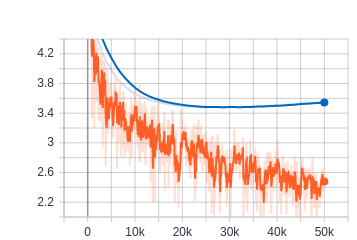
\includegraphics[scale=3.5]{Figure_2}
		
		
	\end{center}
	\caption[Loss - Larger Transformer Model]{Loss - Orange is training loss and blue is evaluation loss.}
	
	%\addcontentsline{lof}{section}{Word Embeddings}
\end{figure}

Subjectively this transformer model is better than the Transformer model based on the smaller hyper-parameter set and the Persona Corpus.


%\begin{lstlisting}[language=bash]
\subsubsection*{Questions}
This is the sample question list as it was answered by the model.

\begin{verbatim}
> Hello.
hello 
> What is your name?
i don't know 
> What time is it?
i don't know 
> What do you do?
what do you mean ?
> What is your favorite color?
i don't know 
> Do you like red?
no 
> Do you like blue?
yeah 
> What is your favorite candy?
i don't know 
> Do you like ice cream?
yeah 
> Good bye.
bye 
\end{verbatim}

\noindent \textbf{Checklist:} 



\begin{itemize}
	
	\item[\rlap{\raisebox{0.3ex}{\hspace{0.4ex}\scriptsize \ding{52}}}$\square$] All the responses are in plain English. There is no gibberish.
	
	\item[\rlap{\raisebox{0.3ex}{\hspace{0.4ex}\scriptsize \ding{52}}}$\square$] There is a variety of answers. Not all answers are the same.
	
	\item[\rlap{\raisebox{0.3ex}{\hspace{0.4ex}\scriptsize \ding{56}}}$\square$] The `favorite color' and `favorite candy' questions are ignored.
	
	\item[\rlap{\raisebox{0.3ex}{\hspace{0.4ex}\scriptsize \ding{56}}}$\square$] The model does in fact use `No' or `I don't know'. It also likes to answer `yeah'.
	
	\item[\rlap{\raisebox{0.3ex}{\hspace{0.4ex}\scriptsize \ding{52}}}$\square$] The model does have an answer for `Good bye'.
\end{itemize}

\subsection{Smart Speaker - Transformer Model with Movie Corpus}

The transformer model is installed on the Raspberry Pi. It takes about five seconds to answer any question.

The transformer model takes about two minutes to boot on the Raspberry Pi. After that the time between responses is slow. The time between the first two or three responses is uncomfortably slow. After those first responses the time between answers gets to be more natural.

There is a special tone that the Raspberry Pi gives at the end of loading the model. This tone notifies the user that the model is loaded and ready to respond to questions. The model is also configured to beep intermittently during operation to signal that it is processing an input. This is helpful for a configuration where there is no monitor.


\subsection{Chatbot - Generative Pre-training Transformer 2 Model}
We used a pre-trained Generative Pre-training Transformer 2 model with the large english corpus to produce a chatbot and ascertain if this model works better than the sequence-to-sequence model. In our tests this worked well. The corpus is called `WebText'.

For our experiments Generative Pre-training Transformer 2 was used for the chatbot model in `zero-shot' mode. This means we did no special fine-tuning of the model in the application.

We did do some special coding for the input and output code in order to operate it as a chatbot. Output was limited to about 25 tokens. 

Input to the model was prepended with the character string "Q:" by our code. Output was observed to have the character string "A:" prepended to it. We assume therefore that the model was at some point exposed to the "Question/Answer" paradigm in written passages during its training. This was helpful.

Output from the model was usually larger in size than we needed. Also, output had the character of having some sensible utterance followed by some output that was only a partial sentence.

It was necessary to `scrape' the output. First the output was checked for the "A:" character string at the start. If it was there it was removed. Then the first complete sentence was used as output, while words and phrases after that were discarded.

\subsubsection{Context Experiment}
We decided that we would attempt to give the model some details that it could draw on during normal execution. We had two choices here. One choice was to train the model using fine-tuning and transfer learning to recognize certain questions and to supply answers. The other choice was to simply show the model the list of facts that we thought were important before every input sequence. This information would be summarized with each reply.

The second choice was more interesting. The text that the model was shown always included the name of the model (picked somewhat arbitrarily) along with information about the location of the model and the occupation. The time was also included.

This worked under most circumstances. Occasionally the model would report the wrong time when asked. This sort of activity is mysterious.

\subsubsection{History Experiment}
We tried concatenating all input and output and including it with each question. The hope was that the model would treat the `Q' and `A' as historical input and then it could refer to that input as it answered new questions. This didn't work, and the model was usually confused by the extra input.

\subsubsection{Artificial Intelligence Markup Language Experiment}
It was deemed helpful if the model could be given a question and instructed how to answer it. To this end AIML files were constructed and an AIML kernel was employed. The user's question was shown to the AIML kernel and then the model was shown the kernel's output (if there was one) along with the original question. The hope was that the output could be controlled by the AIML component. It didn't work. The AIML confused the model, and the model would not reliably choose to answer with the AIML text, as it might with the time of day.

\subsubsection{Overall}

Subjectively the model was the best of those tested. The model would answer questions about it's location, it's name, and the time, faithfully most of the time. Interestingly there where times when it did not do so. Some times it used alternative answers. For example, it would answer with the time but not the correct time. This was odd.

Under almost all circumstances the output was sensible English. There were no times where the model replied with gibberish. 

The subject matter of the prompts did not need to be the same as the simple introductory conversation of the transformer model. In fact any subject matter could be chosen and the model would answer. The model did not remember its own answers but it was consistent. Questions it answered include `What is your favorite color?' and `Do you like lollipops?'. 

\subsubsection*{Questions}
This is the sample question list as it was answered by the model. Note that the information mentioned in the answer about the time was accurate when the test was run.

\begin{verbatim}
> hello
Hello.
> what is your name ?
My name is Jane.
> what time is it ?
02:59 PM January 28, 2020.
> what do you do ?
I am a student.
> what is your favorite color ?
I love the color of the rainbow.
> do you like red ?
Yes.
> do you like blue ?
I do.
> what is your favorite candy ?
I love candy.
> do you like ice cream ?
I do. 
> good bye
Good bye.
\end{verbatim}

\noindent \textbf{Checklist:} 


\begin{itemize}
	
	\item[\rlap{\raisebox{0.3ex}{\hspace{0.4ex}\scriptsize \ding{52}}}$\square$] All the responses are in plain English. There is no gibberish.
	
	\item[\rlap{\raisebox{0.3ex}{\hspace{0.4ex}\scriptsize \ding{52}}}$\square$] There is a variety of answers. Not all answers are the same.
	
	\item[$\square$] It is still debatable weather or not the answers to the questions about `favorite color' and `favorite candy' are good. The model could have a set of answers that it can use for this kind of question. The model seems to know what candy is and to a lesser extent what a color is. Some of the time the answer includes a word from the question sentence that would lead you to believe that this model has fewer stock answers. The answers are good but not perfect.
	
	\item[\rlap{\raisebox{0.3ex}{\hspace{0.4ex}\scriptsize \ding{52}}}$\square$] The model does not use `I don't know' that often. 
	
	\item[\rlap{\raisebox{0.3ex}{\hspace{0.4ex}\scriptsize \ding{52}}}$\square$] The model does have an answer for `Good bye'.
\end{itemize}

The model will answer with it's name and you can tell it your name, but it is confused by this. It will on occasion tell you that it's name and your name are the same thing. This is in part because it cannot remember what it most recently said to you or what you most recently said to it. 

\subsection{Smart Speaker - Generative Pre-training Transformer 2 Model}
Tests showed that the Generative Pre-training Transformer 2 chatbot worked well. We wanted to continue and allow the chatbot to have more of the abilities of a smart speaker. We constructed a simple corpus that contained key phrases that we wanted the chatbot to recognize and act upon. We did some transfer learning with this new corpus.

We found that one of two things would happen. The chatbot would either learn the new phrases and forget all it's pre-training, or it would not learn the new phrases and it would retain all it's pre-training. For our examples there seemed to be no middle ground. Comparisons were made with all available models and a version without the transfer learning was settled on.

Code was added that uses Text To Speech and Speech To Text libraries. In this way the model could interact with a subject using auditory cues and commands.

We did some programming that allowed the model to launch programs when directed to by the user. In this way we have tried to move our project closer to the smart-speakers that are produced commercially. The programming did not rely on the neural-network aspects of the model. Instead the code used heuristics and simple word recognition. This code can be disabled when the model is run from the command line.

The Raspberry Pi model that the Generative Pre-training Transformer 2 was installed on was the 4B with 4GB of RAM. It is largely for this model that we cross compiled the Pytorch Python library for the ARMv7. The GPT2 model fit on the Raspberry Pi. While execution on the production laptop was instantaneous, execution on the Raspberry Pi took about 13 seconds for every response from the neural network.

The Raspberry Pi was outfitted with a microphone and a speaker but no mouse, monitor, or keyboard. The program was modified so that there was a tone every time the model was ready for input. Without such a tone it would be difficult to know when to speak and when to wait for a response. Aesthetically this arrangement is not perfect, but it allows the Generative Pre-training Transformer 2 model to be physically installed on the Raspberry Pi.

\section{Observation}
It is important here to compare the GRU chatbot with the larger Transformer based chatbot. Using our subjective qualifications we see that the GRU model answers with more variety than the transformer model. The important observation is that the hyper-parameter set for the Transformer model can be expanded and enlarged as needed before training. The GRU model cannot be trained successfully with an arbitrarily large hyper-parameter set. We can train a larger Transformer and obtain the benefit associated with this, namely better responses.

A single further observation is that the GRU model responds very quickly, while a transformer model may take more time relatively. This is not a problem for general applications, but for our purposes we cannot ignore the time spent by the transformer model when it is installed on a small computer like a Raspberry Pi. 

The respective value of each of the models changes slightly when you  consider what platform they will be implemented on. The GRU responds more quickly and so it retains more worth.

\section{Tests}

\subsection*{Turing Test}

The Turing Test concerns itself with the question of weather a computer is intelligent. Turing says that intelligence is too hard to describe, and that if the computer can convince you that it is intelligent then it is.

Weather this is right is beyond the scope of this paper. The people who trained the Generative Pre-training Transformer 2 were apprehensive about their model's ability to generate human speech. At first when they finished their model they decided not to release the largest version to the public for several months (Radford et al.)\cite{radford2019language}. Ultimately they did release their large model.

The creators of the model used it differently than our chatbot implementation. They generated paragraphs of text, and it was determined at first that the ability of the model to impersonate a human was too great. It was felt that the model could be used to spam facebook and other social networking sites with content that was very convincing. If the model could be used to convince people to act badly, then it should not be released. Humans are susceptible to the sentiments of those they see as their peers. If the model was, for better or worse, passing the Turing test, then it should not fall into the wrong hands. This was the concern of the coders at the time.

Ultimately the large model was released, either because the developers decided the model was not as good as originally estimated, or because they didn't care. 

\subsection*{Winograd Schema}

Winograd schemas are named after Terry Winograd. The idea is that there is a sentence presented that has two meanings. A computer finds these sentences challenging to understand, and that makes them interesting for the development of Artificial Intelligence.

An example follows.

\begin{center}
	\textbf{He didn't put the trophy in the suitcase because it was too [big/small]}
\end{center}

We can choose which bracketed term to use, and we must choose only one bracketed term. If we choose `big' then we are referring to the trophy. If we choose `small' then we are referring to the suitcase. Human beings can easily see the pronoun `it' refers to either the suitcase or the trophy. Computers have trouble with these determinations.

The Transformer, and the Scaled Dot-product Attention that it uses, lends itself to discussion of Winograd schema. In the chat bot example, we are less interested in the Winograd example because it doesn't come up often. However, in the case of the Generative Pre-training Transformer 2, and it's exhaustive training, it is interesting to consider the Winograd style example sentences.

There is a Winograd Schema Challenge and something of a formula for constructing your own Winograd schema (Wikapedia contributors, 2020). \cite{wiki:xxx}

